\documentclass[pdflatex,sn-basic]{sn-jnl}
\usepackage{amsmath,amssymb,booktabs,graphicx}
\graphicspath{{figures/}}
\renewcommand{\thetable}{S\arabic{table}}
\renewcommand{\thefigure}{S\arabic{figure}}
\begin{document}
\title{Online Resource 1 for ``What can country panels tell us about broadband price responsiveness? Evidence from the European Union and the Eastern Partnership, 2010--2024''}
\abstract{This Online Resource reports additional estimates and the data-construction details referred to in the article. All estimates can be reproduced from public data with the code in the replication package.}
\maketitle
\section*{Additional tables}
\begin{table}[h]
\caption{First-difference estimates, 2010--2019: pooled, EU and EaP coefficients under alternative choices}\label{tab:S1}
\footnotesize\setlength{\tabcolsep}{4pt}
\begin{tabular*}{\textwidth}{@{\extracolsep{\fill}}lccccccc@{}}
\toprule
& \multicolumn{2}{c}{Pooled} & \multicolumn{2}{c}{EU} & \multicolumn{2}{c}{EaP} & \\
\cmidrule(lr){2-3}\cmidrule(lr){4-5}\cmidrule(lr){6-7}
Specification & Coef. & SE & Coef. & SE & Coef. & SE & Obs.\\
\midrule
Baseline & $-0.07^{*}$ & (0.04) & $-0.01$ & (0.02) & $-0.28^{***}$ & (0.08) & 240\\
Price in PPP dollars & $-0.03$ & (0.03) & $-0.02$ & (0.02) & $-0.10$ & (0.23) & 233\\
Price in current US dollars & $-0.06$ & (0.04) & $-0.02$ & (0.02) & $-0.23^{*}$ & (0.12) & 242\\
GDP only & $-0.07^{*}$ & (0.04) & $-0.01$ & (0.02) & $-0.27^{***}$ & (0.07) & 240\\
+ servers and R\&D & $-0.06$ & (0.04) & $0.00$ & (0.02) & $-0.25^{***}$ & (0.09) & 240\\
+ mobile basket (2014--19) & $-0.01$ & (0.01) & $-0.01$ & (0.01) & $-0.02$ & (0.04) & 140\\
Internet users outcome & $-0.08^{***}$ & (0.03) & $-0.03^{*}$ & (0.01) & $-0.27^{***}$ & (0.03) & 240\\
Incl.\ repeated 2019, 2017--18 & $-0.06^{*}$ & (0.03) & $-0.01$ & (0.01) & $-0.27^{***}$ & (0.08) & 295\\
Log count of subscriptions & $-0.06^{*}$ & (0.03) & $-0.01$ & (0.01) & $-0.26^{***}$ & (0.08) & 295\\
Sample ending in 2017 & $-0.09^{*}$ & (0.05) & $-0.01$ & (0.02) & $-0.28^{***}$ & (0.08) & 229\\
Log-odds, $K=55$ & $-0.08^{*}$ & (0.04) & $-0.02$ & (0.02) & $-0.31^{***}$ & (0.09) & 240\\
Log-odds, $K=70$ & $-0.08^{*}$ & (0.04) & $-0.01$ & (0.02) & $-0.30^{***}$ & (0.08) & 240\\
Log-odds, $K=100$ & $-0.07^{*}$ & (0.04) & $-0.01$ & (0.02) & $-0.29^{***}$ & (0.08) & 240\\
Driscoll--Kraay SEs & & & $-0.01$ & (0.01) & $-0.28^{***}$ & (0.08) & 240\\
\botrule
\end{tabular*}
\footnotetext{First differences with year effects and core controls; clustered standard errors unless stated. Log-odds rows use $\ln[s/(K-s)]$ as the outcome. The mobile-broadband basket is available from 2013, which restricts the differenced sample to 2014--2019. Driscoll--Kraay: Bartlett kernel, bandwidth 3. $^{*}p<0.10$, $^{**}p<0.05$, $^{***}p<0.01$.}
\end{table}

\begin{table}[h]
\caption{Functional form and headroom, first differences, 2010--2019}\label{tab:S2}
\footnotesize
\begin{tabular*}{\textwidth}{@{\extracolsep{\fill}}lcccc@{}}
\toprule
\multicolumn{5}{@{}l}{\textit{Panel A. Implied elasticity at group means}}\\
Form & EU & $p$ & EaP & $p$ \\
\midrule
Linear ($s$ on price) & $-0.00$ & 0.852 & $-0.04$ & 0.277\\
Log-linear ($\ln s$ on price) & $0.00$ & 0.952 & $-0.21$ & 0.000\\
Linear-log ($s$ on $\ln$ price) & $-0.01$ & 0.507 & $-0.12$ & 0.114\\
\midrule
\multicolumn{5}{@{}l}{\textit{Panel B. Price coefficient varying with headroom $h_{i,t-1}=1-s_{i,t-1}/70$ (centred)}}\\
& \multicolumn{2}{c}{2010--2019} & \multicolumn{2}{c}{2010--2024}\\
$\Delta\ln p$ & $-0.02$ (0.02) & & $-0.04^{***}$ (0.02) & \\
$\Delta\ln p\times h$ & $-0.69^{*}$ (0.35) & & $-0.49^{*}$ (0.28) & \\
$\Delta\ln p\times$ post-2019 & & & $0.02$ (0.02) & \\
\multicolumn{5}{@{}l}{\textit{Adding the EaP interaction (2010--2019)}}\\
$\Delta\ln p$; $\times$EaP; $\times h$ & \multicolumn{4}{l}{$-0.00$ (0.02);\quad $-0.23^{***}$ (0.05);\quad $-0.19$ (0.29)}\\
\botrule
\end{tabular*}
\footnotetext{Panel A: elasticities evaluated at group mean price and penetration; $p$-values refer to the underlying coefficient (EaP: sum of main and interaction terms). Panel B: clustered standard errors in parentheses. $^{*}p<0.10$, $^{**}p<0.05$, $^{***}p<0.01$.}
\end{table}

\begin{table}[h]
\caption{Price $\times$ post-2019: sample restrictions}\label{tab:S3}
\footnotesize
\begin{tabular*}{\textwidth}{@{\extracolsep{\fill}}lccccc@{}}
\toprule
& \multicolumn{2}{c}{TWFE levels} & \multicolumn{2}{c}{First differences} & \\
\cmidrule(lr){2-3}\cmidrule(lr){4-5}
Sample & Price & Price $\times$ post & Price & Price $\times$ post & Obs. (FD)\\
\midrule
Full sample & $-0.22^{***}$ & $0.30^{***}$ & $-0.07^{**}$ & $0.05^{**}$ & 382\\
 & (0.05) & (0.07) & (0.03) & (0.02) & \\
Excl.\ UKR 2022--24, BLR 2020--24 & $-0.23^{***}$ & $0.29^{***}$ & $-0.06^{*}$ & $0.05^{**}$ & 375\\
 & (0.05) & (0.07) & (0.03) & (0.02) & \\
Ending in 2021 & $-0.21^{***}$ & $0.27^{***}$ & $-0.07^{*}$ & $0.06$ & 284\\
 & (0.06) & (0.07) & (0.04) & (0.03) & \\
\botrule
\end{tabular*}
\footnotetext{Core controls; country and year effects (levels) or year effects (first differences); clustered standard errors. $^{*}p<0.10$, $^{**}p<0.05$, $^{***}p<0.01$.}
\end{table}

\begin{table}[h]
\caption{Hausman-type instrumental-variable estimates, pooled}\label{tab:S4}
\footnotesize
\begin{tabular*}{\textwidth}{@{\extracolsep{\fill}}llccc@{}}
\toprule
Estimator & Instrument & Coef. (SE) & First-stage $F$ & Anderson--Rubin 95\% set\\
\midrule
Levels, 2010--2019 & sub-regional & -1.31 (0.46) & 12.0 & [-3.2, -0.6]\\
Levels, 2010--2019 & 3 nearest capitals & -2.18 (1.51) & 2.5 & [-6.0, -0.4] (grid edge)\\
FD, 2010--2019 & sub-regional & 1.81 (2.30) & 1.0 & --\\
FD, 2010--2019 & nearest capitals & 0.96 (0.93) & 2.1 & --\\
FD, 2010--2019 & both & 1.03 (1.01) & 2.1 & --\\
FD, 2010--2024 & sub-regional & 61.40 (2072.53) & 0.0 & --\\
FD, 2010--2024 & nearest capitals & 0.95 (0.87) & 2.1 & --\\
FD, 2010--2024 & both & 0.49 (0.49) & 2.4 & --\\
\botrule
\end{tabular*}
\footnotetext{Instruments are averages of log prices of other sample countries in the same year: the leave-one-out mean of the country's sub-region, or the inverse-distance-weighted mean of the three countries with the nearest capitals. Levels regressions are two-way demeaned; FD regressions include year effects. Core controls; standard errors clustered by country. The Anderson--Rubin (AR) set was computed on a grid over $[-6,4]$. Sub-regions: Nordic (DNK, FIN, SWE), Baltic (EST, LVA, LTU), Western (AUT, BEL, DEU, FRA, IRL, LUX, NLD), Southern (CYP, ESP, GRC, ITA, MLT, PRT), Central (CZE, HUN, POL, SVK), South-Eastern (BGR, HRV, ROU, SVN), South Caucasus (ARM, AZE, GEO), Eastern (BLR, MDA, UKR). The first-difference first stages are too weak for the estimates to be informative.}
\end{table}

\begin{table}[h]
\caption{Country-specific first-difference slopes (2010--2019) and weights in the levels regression}\label{tab:S5}
\footnotesize
\begin{tabular*}{\textwidth}{@{\extracolsep{\fill}}lcccc|lcccc@{}}
\toprule
Country & Slope & SE & Obs. & TWFE weight & Country & Slope & SE & Obs. & TWFE weight\\
\midrule
LTU & -0.27 & 0.18 & 7 & 0.015 & HRV & 0.01 & 0.01 & 8 & 0.063\\
CZE & -0.20 & 0.06 & 7 & 0.021 & LUX & 0.01 & 0.08 & 7 & 0.005\\
PRT & -0.17 & 0.15 & 7 & 0.011 & BEL & 0.01 & 0.03 & 7 & 0.021\\
FIN & -0.06 & 0.08 & 7 & 0.011 & DNK & 0.02 & 0.07 & 7 & 0.004\\
BGR & -0.04 & 0.10 & 7 & 0.010 & MLT & 0.02 & 0.02 & 7 & 0.038\\
DEU & -0.03 & 0.03 & 7 & 0.005 & ESP & 0.03 & 0.09 & 8 & 0.041\\
NLD & -0.03 & 0.04 & 8 & 0.010 & HUN & 0.05 & 0.10 & 7 & 0.023\\
GRC & -0.02 & 0.06 & 7 & 0.022 & SWE & 0.08 & 0.09 & 7 & 0.023\\
POL & -0.02 & 0.08 & 7 & 0.043 & ROU & 0.12 & 0.45 & 5 & 0.012\\
CYP & -0.02 & 0.02 & 7 & 0.027 & EST & 0.17 & 0.13 & 7 & 0.014\\
AUT & -0.02 & 0.05 & 8 & 0.019 & \textbf{AZE} & -0.75 & 0.34 & 7 & 0.025\\
IRL & -0.02 & 0.02 & 7 & 0.055 & \textbf{ARM} & -0.41 & 0.16 & 7 & 0.155\\
LVA & -0.00 & 0.04 & 8 & 0.044 & \textbf{MDA} & -0.41 & 0.23 & 7 & 0.009\\
SVN & -0.00 & 0.03 & 8 & 0.021 & \textbf{BLR} & -0.21 & 0.11 & 7 & 0.084\\
SVK & 0.01 & 0.05 & 8 & 0.016 & \textbf{UKR} & -0.05 & 0.21 & 8 & 0.031\\
ITA & 0.01 & 0.04 & 8 & 0.081 & \textbf{GEO} & 0.67 & 0.42 & 8 & 0.020\\
FRA & 0.01 & 0.03 & 8 & 0.021 & & & & &\\
\botrule
\end{tabular*}
\footnotetext{Slopes: regression of the annual change in log subscriptions per 100 on the change in log price and log GDP per capita with a constant, by country; conventional standard errors. EaP countries in bold. TWFE weight: country's share of the sum of squared residualised prices in the 2010--2019 levels regression (price residualised on country and year effects and core controls); the six EaP countries account for 32\%.}
\end{table}

\begin{table}[h]
\caption{Data construction: flags, imputations and sample composition}\label{tab:S6}
\footnotesize
\begin{tabular*}{\textwidth}{@{\extracolsep{\fill}}p{4.2cm}p{8.2cm}@{}}
\toprule
Item & Treatment \\
\midrule
ITU basket definition & 1\,GB minimum (2010--2017), 5\,GB minimum (2018--2024); the 2017--2018 change is never used in differenced regressions.\\
2019 prices equal to 2018 in all three units & 22 countries (ARM, AZE, BEL, BGR, BLR, CYP, CZE, DEU, DNK, EST, FIN, GRC, HUN, IRL, LTU, LUX, MDA, MLT, POL, PRT, ROU, SWE); set to missing.\\
Missing in source & Romania 2013 price; Bulgaria 2024 subscriptions; left missing.\\
Mobile-broadband basket & Chain of ITU data-only baskets: postpaid computer-based 1\,GB (2013--2017), 1.5\,GB (2018--2020), 2\,GB (2021--2024).\\
Tertiary enrolment & 9 interior values interpolated, 21 end values set to nearest observation.\\
R\&D expenditure (robustness only) & 30 end values set to nearest observation.\\
Population density & 2024 values computed from population and land area.\\
Night-time lights & Harmonised DMSP (to 2013) and simulated VIIRS (from 2014) radiance summed over Natural Earth national boundaries (European France only); the 2013--2014 change is excluded.\\
First-difference observations by year & 2011: 33, 2012: 33, 2013: 32, 2014: 32, 2015: 33, 2016: 33, 2017: 33, 2019: 11, 2020: 11, 2021: 33, 2022: 33, 2023: 33, 2024: 32.\\
Earlier version of this panel & Used $\ln(1+p)$ instead of $\ln p$, forward-filled missing prices and subscriptions, and averaged different mobile baskets; all corrected here.\\
\botrule
\end{tabular*}
\end{table}

\begin{table}[h]
\caption{EaP first-difference coefficient by year and identification checks, 2010--2019}\label{tab:S7}
\footnotesize
\begin{tabular*}{\textwidth}{@{\extracolsep{\fill}}lccc@{}}
\toprule
\multicolumn{4}{@{}l}{\textit{Panel A. EaP coefficient by year (common EU slope, year effects, core controls)}}\\
Year & Coef. & SE & EaP countries with data\\
\midrule
2011 & $-0.75$ & (0.20) & 6\\
2012 & $-0.07$ & (0.23) & 6\\
2013 & $-0.61$ & (0.26) & 6\\
2014 & $-0.28$ & (0.11) & 6\\
2015 & $-0.58$ & (0.22) & 6\\
2016 & $-0.24$ & (0.14) & 6\\
2017 & $-0.08$ & (0.06) & 6\\
2019 & $0.80$ & (0.19) & 2\\
\midrule
\multicolumn{4}{@{}l}{\textit{Panel B. Alternative fixed effects in first differences}}\\
Specification & EU & EaP & WCR $p$ (difference)\\
Year effects (baseline) & $-0.01$ & $-0.28^{***}$ & 0.037\\
Year and country effects & $-0.00$ & $-0.17^{**}$ & 0.133\\
Group-specific year effects & $-0.00$ & $0.13$ & 0.523\\
\botrule
\end{tabular*}
\footnotetext{Panel A: coefficient on the change in log price for EaP countries in each year, from one regression in which the EaP slope is year-specific and the EU slope common; 2018 is omitted because of the basket revision, and in 2019 only two EaP countries report a new price. Panel B: first-difference models of Table 4 in the article; with group-specific year effects the EaP coefficient is identified only from differences among EaP countries within a year. $^{*}p<0.10$, $^{**}p<0.05$, $^{***}p<0.01$.}
\end{table}

\begin{figure}[h]
\centering
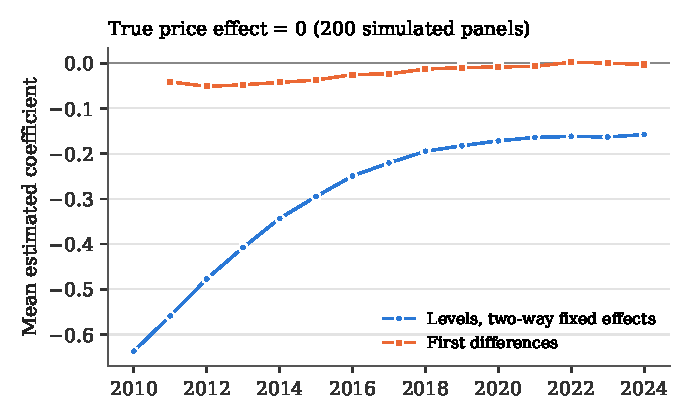
\includegraphics[width=0.7\textwidth]{figS1_simulation.pdf}
\caption{Simulated year-specific coefficients when the true price coefficient is zero. 33 countries follow logistic adoption paths (ceilings 35--50 per 100, speeds 0.25--0.45); 27 have diffusion midpoints before the sample (mean $-4$ years), six start late (mean midpoint in year 3) with affordability ratios about 1.3 log points higher that fall with the stage of diffusion. Idiosyncratic noise: 0.03 in log adoption, 0.15 in log price. Lines show means over 200 panels of the year-specific coefficients from the levels regression with country and year effects and from first differences with year effects. The pooled coefficients average $-0.48$ (levels) and $-0.02$ (first differences)}\label{fig:S1}
\end{figure}

\end{document}
